\chapter{Key Structures}
\label{chapter3}

In this project, we build a sequence-to-sequence (seq2seq) model using LSTM encoders and decoders with which is similar to the seq2seq model described in \cite{bahdanau2014neural}. The seq2seq model is also known as encoder-decoder model, which are widely used in machine translation from a source language to a target language. Thus, the encoder-decoder model can also be used for GEC task, where the encoder network can be used for encoding the potentially error source sentences in the vector space and the decoder network can be used for generating the corrected output sentences by using the source encoding, saying that we treat the error  sentences as the source language and treat the corresponding correct sentence as another language (the target language).

\section{Problem Formulation}
In the part, we will apply the theoretic tool to formulate the GEC problem, which can become a good base for the later analysis and problem solution description. By using the tools of the probabilistic theory and optimization theory, the GEC task problem can be formulated as the following problem, where the designers are requested to find a correct sentence $\mathbf{y}$ that maximizes the conditional probability of the case where the correct sentence is $\mathbf{y}$ given a source sentence $\mathbf{x}$, i.e.,

$${\rm argmax}_\mathbf{y}p\left(\mathbf{y}| \mathbf{x}\right).$$

In order to get a proper neural network model, we need to train a parameterized model which can maximize the conditional probability of the case where the correct sentence is $\mathbf{y}$ given a source sentence $\mathbf{x}$, using a parallel training corpus (source input words and target input words as shown in Figure~\ref{fig:4}). Once the conditional distribution is learned by the model (a translation model), given a source sentence a corresponding correction can be generated by searching for the sentence that maximizes the conditional probability.

\begin{figure}[ht]
    \centering
    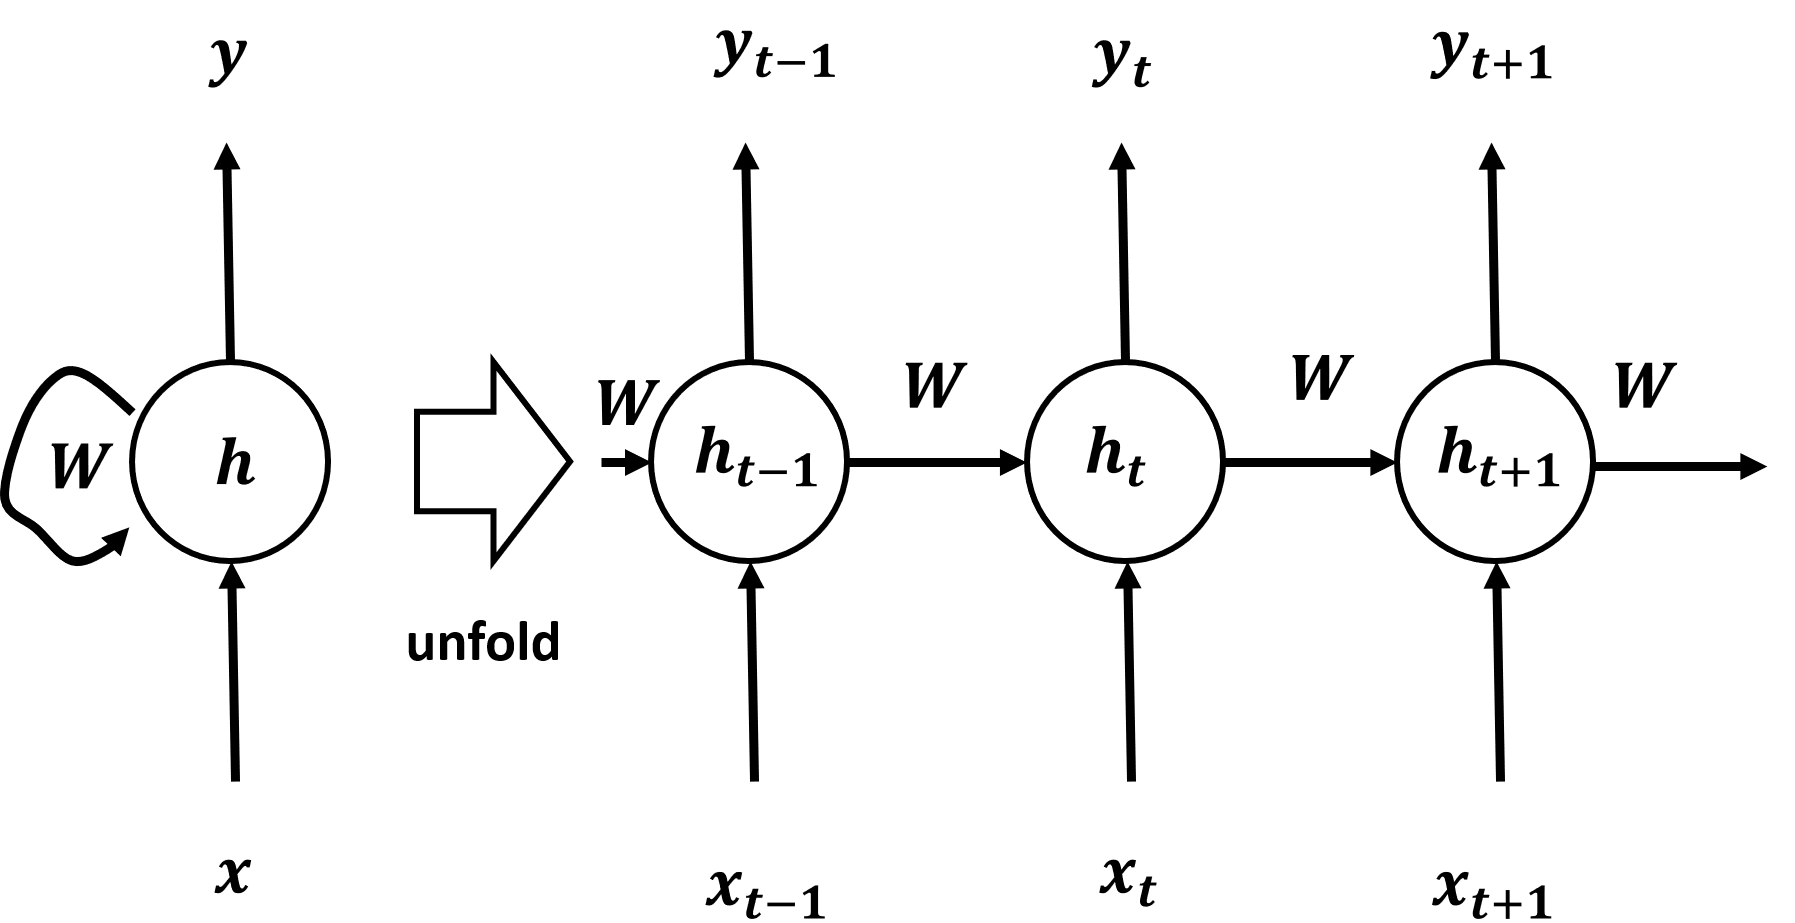
\includegraphics[width=\textwidth]{RNN.png}
    \caption{A recurrent neural network and the unfolding in time of the computation involved in its forward computation.}
    \label{fig:4}
\end{figure}

\section{RNN Encoder–Decoder}

In this part, we will describe briefly the underlying framework, called RNN Encoder–Decoder, which is originally proposed by \cite{cho2014learning,sutskever2014sequence}. The novel architecture we build is also based on the above RNN Encoder–Decoder. Thus, it is necessary to have a detailed description about the RNN Encoder-Decoder model. In this model, there are two RNN, one of which is responsible for encoding the input sequence into a fixed length vector representation and another of which is responsible for decoding that representations into another sequence of symbols. Usually, they are jointly trained to maximize the conditional probability of the target sequence $\mathbf{y}$ given the input sequence $\mathbf{x}$ and the standard log loss of recurrent neural network is used to improve empirical performance. This part will provide a detailed description on RNN and seq2seq model which will be used in our built model.

\subsection{Preliminary: Recurrent Neural Networks}
The insights behind RNNs is to make full utilization of the sequential information of the input data. For a traditional neural network, we know before, we usually make an assumption that all input samples (or even the output data) should be independent of each other. But in many real tasks, that assumption is not a good idea. For example, if you want to predict the next word in a sentence, you had better to know the words that come before it. In this example, the input words are dependent on the words before them, which is beyond the assumption of the traditional neural networks. For this requirement, RNNs are proposed. RNNs are called recurrent for the fact that they do the same task for every element of a sequence and output a result which is dependent on the previous computations. In other word, we can think about RNNs that they have a “memory” which store the information about what has been calculated so far. From theoretic aspects, RNNs can make use of information in arbitrarily-length sequences. However, in practice, RNNS are limited to looking back just only a few steps. The following will give a theoretical formulation of the RNNs which is shown in Figure~\ref{fig:4}.

According to \cite{cho2014learning}, the recurrent neural network (RNN) is a special kind of neural network, which consists of a hidden state $\mathbf{h}$ and an optional output $\mathbf{y}$ which operates on a variable-length sequence $x=\left(x_1,\ldots,x_T\right)$. At each time step t, the hidden state $\mathbf{h}_{<t>}$ of the RNN is updated by 
$$\mathbf{h}_{<t>}=f\left(\mathbf{h}_{<t-1>},x_t\right),$$
where $f$ is a non-linear activation function. $f$ can be any kind of functions, saying that $f$ may be as simple as an element-wise logistic sigmoid function or even as complex as a long short-term memory (LSTM) unit. An RNN can be trained to learn the probability distribution over a sequence to predict the next symbol in the sequence. In that case, at each timestep $t$, the output is the conditional distribution $p\left(x_t| x_{t-1},\ldots,x_1\right)$, where $(x_{t-1},\ldots,x_1)$ is the previous sequence and $x_t$ is the current symbol we need to predict. For example, we can consider a multi-nomial distribution (1-of-K coding) can be output by using a softmax activation function. The probability of the value of each current element can be expressed as the following
$$p\left(x_{t,j}=1| x_{t-1},\ldots,x_1\right)=\frac{\exp(\mathbf{w}_j\mathbf{h}<t>)}{\sum_{j'=1}^{K}\exp(\mathbf{w}_{j'}\mathbf{h}<t>)},$$
for all possible symbol $j=1,\ldots,K$, where $\mathbf{w}_j$ are the rows of a weight matrix $\mathbf{W}$. By combining these probabilities, we can compute the probability of the sequence $\mathbf{x}$ using
$$p\left(x\right)=\prod_{t=1}^{T}{p\left(x_t=1 | x_{t-1},\ldots,x_1\right)}.$$
From this learned distribution, it is straightforward to sample a new sequence by iteratively sampling a symbol at each time step.

\subsection{Seq2seq Model}

Seq2seq model is a type of RNNs, which has been applied in many area now, such as machine translation, speech recognition, video captioning, etc. This model was first introduced by google in their machine translation system \cite{sutskever2014sequence}, which was shown to outperform all the existing state of arts at that time. Before that, the translation worked in a very naive way which is that each word that users use to type was converted to its target language giving no regard to its grammar and sentence structure. From this aspect, the seq2seq model revolutionized the process of translation by making use of deep learning. Because It not only considers the current word/input while translating but also its neighboring word in the sentences, which is really a big step.

In the Seq2seq framework, an encoder reads the input sentence, a sequence of vectors $x=\left(x_1,\ldots,x_T\right)$, into vector c. Although most of the previous works use to encode a variable-length input sentence into a fixed-length vector, e.g., \cite{cho2014learning}, it is not necessary actually. The most common approach is to use an RNN such that
$$\mathbf{h}_{<t>}=f\left(\mathbf{h}_{<t-1>},x_t\right)$$
and
$$c=q\left(\left\{h_1,\ldots,h_T\right\}\right),$$
where $h_t\in\mathbf{R}^n$  is a hidden state at time $t$, and $c$ is a vector generated from the sequence of the hidden states. $f$ and $q$ are some nonlinear functions. We use LSTM as $f$ and 
$$q\left(\left\{h_1,\ldots,h_T\right\}\right)=h_t.$$
The decoder is often trained to predict the next word $y_{t’}$ given the context vector $c$ and all the previously predicted words 
$$y_1,\ldots,y_{t’}.$$
In other words, the decoder defines a probability over the correction $\mathbf{y}$ by decomposing the joint probability into the ordered conditionals:
$$p\left(\mathbf{y}\right)=\prod_{t=1}^{T}{p\left(y_t|\left\{y_{t-1},\ldots,y_1\right\},c\right)},$$
where 
$$\mathbf{y}=(y_1,\ldots,y_T).$$
With an RNN, each conditional probability is modeled as
$$p\left(y_t|\left\{y_{t-1},\ldots,y_1\right\},c\right)=g\left(y_{t-1},s_t,c\right),$$
where $g$ is a nonlinear, potentially multi-layered, function that outputs the probability of $y_t$, and $s_t$ is the hidden state of the RNN.
Usually, the two components, i.e., encoder and decoders, of the seq2seq model are jointly trained to maximize the conditional log-likelihood
$$\max_\mathbf{\theta}{\frac{1}{N}\sum_{n=1}^{N}{\log{p_\mathbf{\theta}}\left(\mathbf{y}_n\middle|\mathbf{x}_n\right)}}$$
where $\mathbf{\theta}$ is the model parameter set and the $(\mathbf{x}_n,\mathbf{y}_n)$ is the (input sequence, output sequence) pair from the training set.

\begin{figure}[ht]
    \centering
    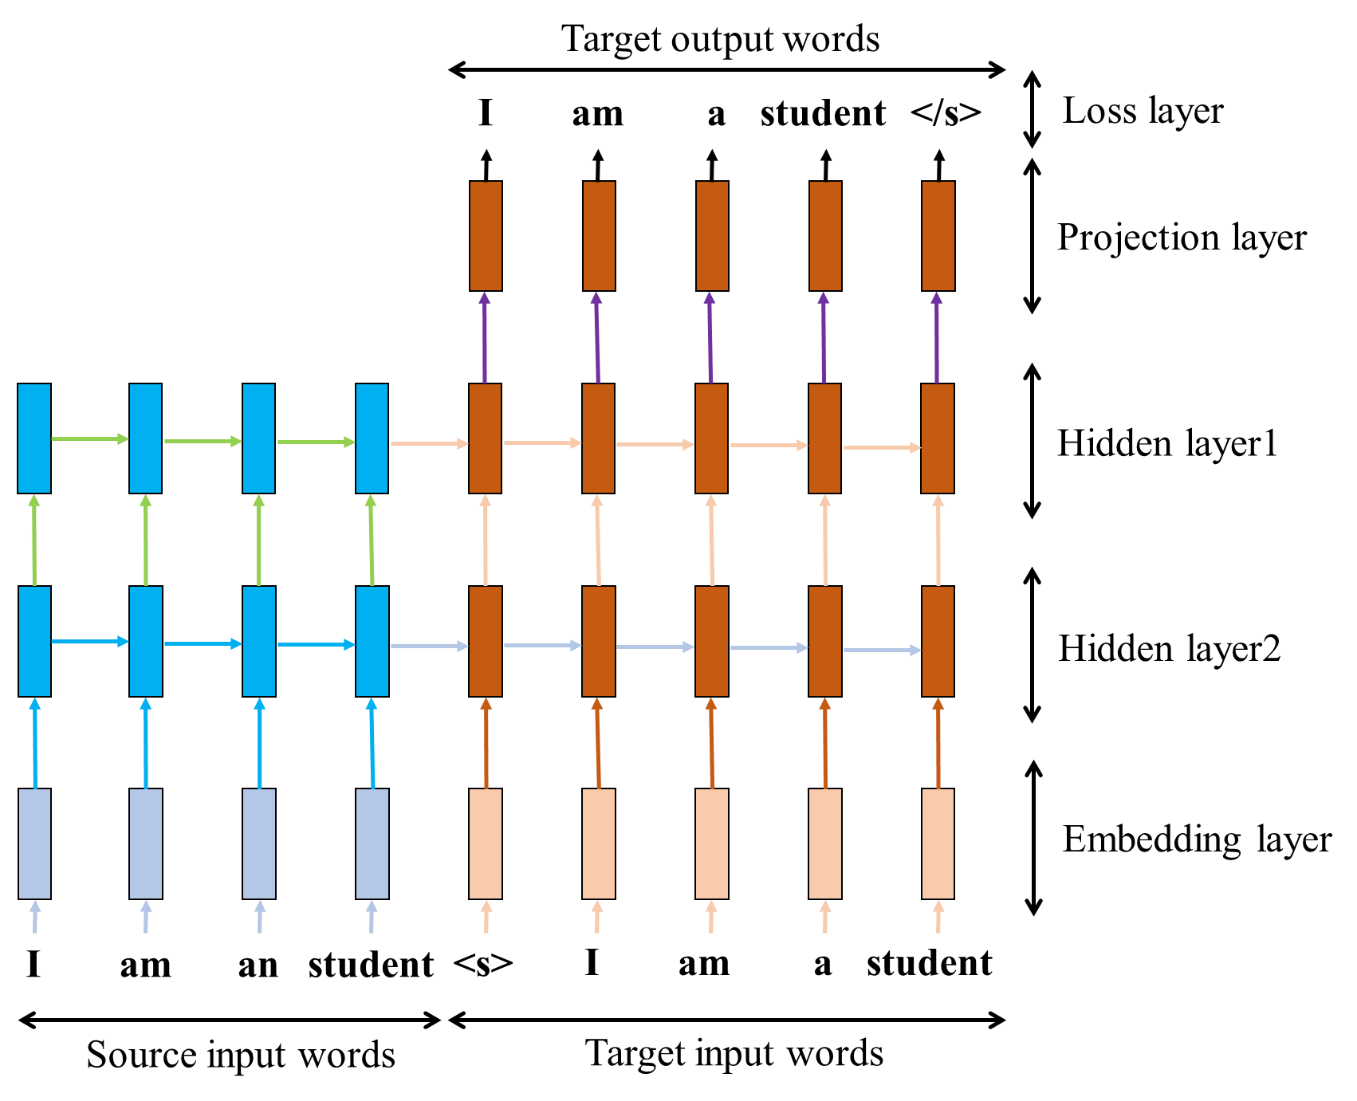
\includegraphics[width=\textwidth]{NMC.png}
    \caption{Neural Machine Correction – example of a deep recurrent architecture proposed by for correct a source sentence "I am an student" into a target sentence " I am a student ". Here, "<s>" marks the start of the decoding process while "</s>" tells the decode.}
    \label{fig:4}
\end{figure}

